\begin{marginfigure}
	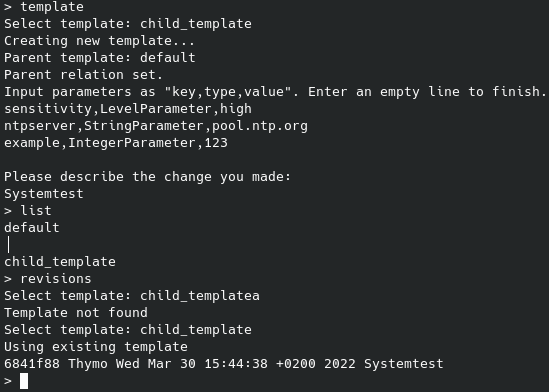
\includegraphics{manage_template}
	\caption{System test 1 result}
	\label{test:2}
\end{marginfigure}

\begin{test}[label={test_camera}]{Managing a template}
	The application should be able to add new templates and configure parameters.
\tcbline
	\begin{description}
		\item[Requirements:] B1, B4, U3, U5, U6, U7, NF8
		\item[Test passes when:] \hfill
			\begin{itemize}
				\item Template can be created.
				\item Parameters can be added to a template.
				\item Template can have a parent associated with it.
				\item Changes are saved inside a revision.
			\end{itemize}
		\item[Result:] Passed (Figure \ref{test:2})
	\end{description}
\end{test}

\begin{marginfigure}
	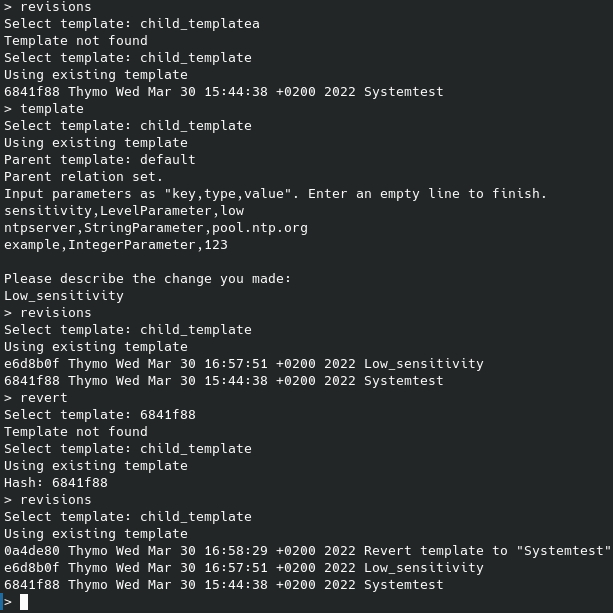
\includegraphics{revert}
	\caption{System test 2 result}
	\label{test:3}
\end{marginfigure}

\begin{test}[label={test_camera}]{Reverting a template}
It should be able to revert a template to a previous revision.\\
\tcbline
	\begin{description}
		\item[Requirements:] B2, B3, U2
		\item[Test passes when:] \hfill
			\begin{itemize}
				\item Revisions and audit information of a template can be displayed.
				\item A new revision can be made by editing a template.
				\item A template can be reverted to an earlier revision.
			\end{itemize}
		\item[Result:] Passed (Figure \ref{test:3})
	\end{description}
\end{test}

\begin{marginfigure}
	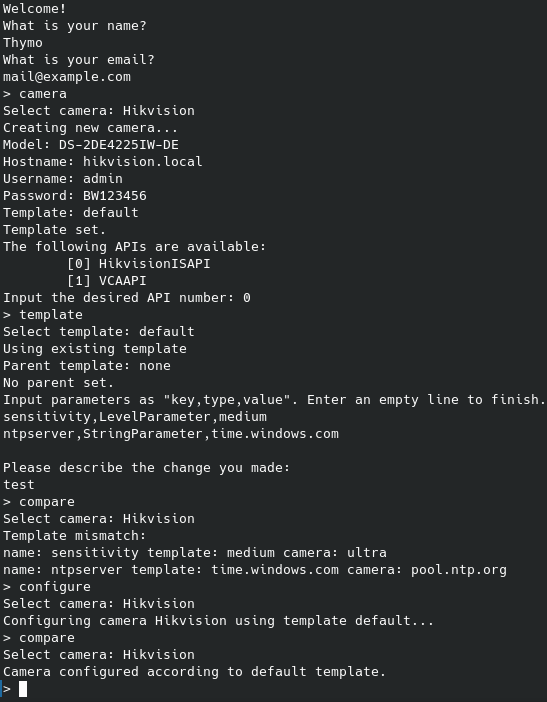
\includegraphics{hikvision_configure}
	\caption{System test 3 result}
	\label{test:4}
\end{marginfigure}

\begin{test}[label={test_hikvision}]{Hikvision support}
It should be possible to read and write the NTP and motion detection sensitivity parameters from the Hikvision camera.
Using this information the compare command should show any mismatches with the template and allow for these to be corrected using the configure command.
\tcbline
	\begin{description}
		\item[Requirements:] B1, B4, B5, U3, U7, U8, U9, NF1, NF8
		\item[Test passes when:] \hfill
			\begin{itemize}
				\item Two parameters supported by the camera can be set in a template.
				\item A mismatch is displayed when the camera value differs from the template.
				\item The parameters from the template can be transferred using the configure command.
				\item Proper updating of the parameters is confirmed by a second compare command.
			\end{itemize}
		\item[Result:] Passed (Figure \ref{test:4})
	\end{description}
\end{test}

\begin{marginfigure}
	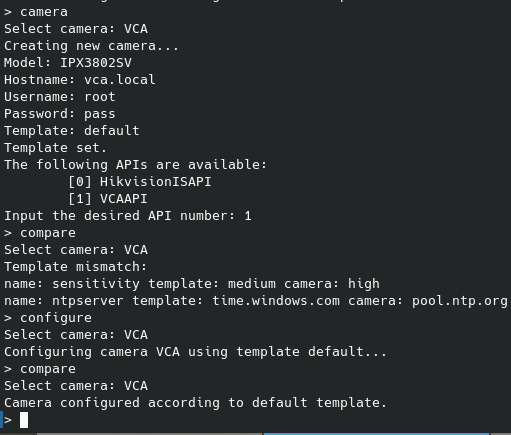
\includegraphics{vca_configure}
	\caption{System test 4 result}
	\label{test:5}
\end{marginfigure}

\begin{test}[label={test_vca}]{VCA support}
It should be possible to read and write the NTP and motion detection sensitivity parameters from the Hikvision camera.
Using this information the compare command should show any mismatches with the template and allow for these to be corrected using the configure command.
\tcbline
	\begin{description}
		\item[Requirements:] B1, B4, B5, U3, U7, U8, U9, NF1, NF8
		\item[Test passes when:] \hfill
			\begin{itemize}
				\item Two parameters supported by the camera can be set in a template.
				\item A mismatch is displayed when the camera value differs from the template.
				\item The parameters from the template can be transferred using the configure command.
				\item Proper updating of the parameters is confirmed by a second compare command.
			\end{itemize}
		\item[Result:] Passed (Figure \ref{test:5})
	\end{description}
\end{test}

\begin{marginfigure}
	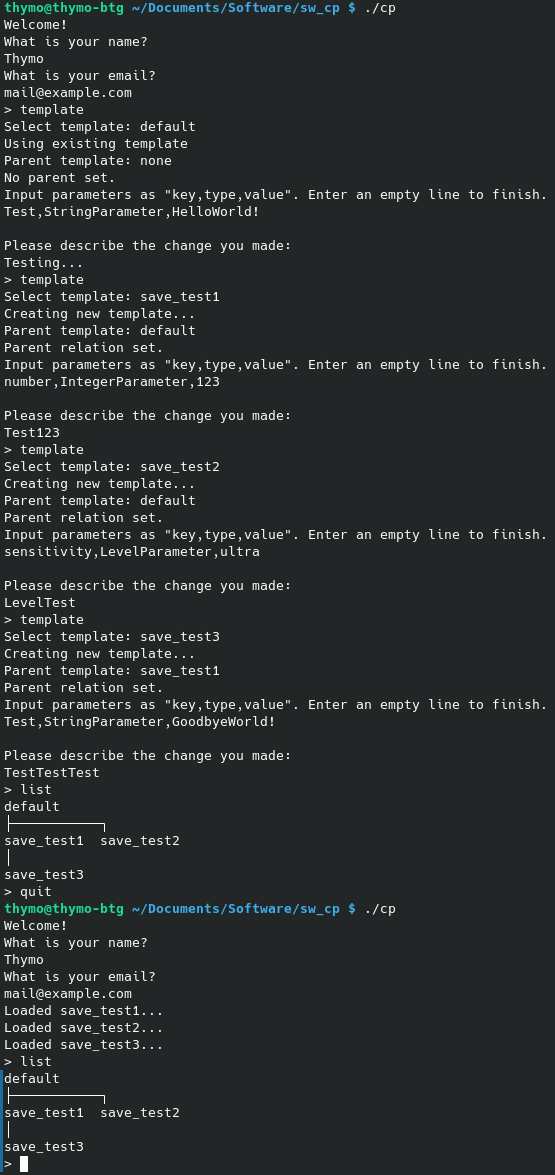
\includegraphics{test_reload}
	\caption{System test 5 results}
	\label{test:6}
\end{marginfigure}

\begin{test}[label={test_camera}]{Saving and loading}
The application should be able to reload the templates that were previously saved when the application is started.
\tcbline
	\begin{description}
		\item[Requirements:] NF6, NF8
		\item[Test passes when:] \hfill
			\begin{itemize}
				\item Multiple templates containing a parameter are created.
				\item Template hierarchy can be shown before and after restarting the program.
				\item Templates are automatically reloaded.
				\item Hierarchy is preserved across restarts.
			\end{itemize}
		\item[Result:] Passed (Figure \ref{test:6})
	\end{description}
\end{test}
